\section{数据预处理}
\subsection{掩模构建与形态学去噪}
对于花苗图像,我们可以看到,花苗的背景通常为黄土、砂砾或塑料箱等,而绿色的花苗则显得非常好辨认。而且我们面对的花苗是绿色的,因而考虑设置一个hsv范围,将绿色的部分从图像中剥离出来。于是我们首先将花苗图像进行颜色空间的转换,从rgb颜色空间转化为hsv颜色空间,之后设定hsv颜色空间为[26,43,46]和[99,255,255],在原图中过滤出在这个hsv颜色空间的图像得到掩膜,若在这个区间中,则为白色,否则为黑色。之后可以通过该掩膜对原图进行位运算,则可得到原图的图像。其部分代码如下
\begin{lstlisting}[language=python]
import cv2
# 假设待处理的图像为img
# rgb图像转化为hsv图像
hsv = hsv = cv2.cvtColor(img,cv2.COLOR_BGR2HLS)
# 绿色的阈值(HSV)
lower_green = np.array([26,43,46])
upper_green = np.array([99,255,255])
# 根据阈值构建掩膜
mask = cv2.inRange(hsv,lower_green,upper_green)
# 对原图像和掩膜进行位运算
res = cv2.bitwise_and(img,img,mask=mask)
\end{lstlisting}
得到的结果如下,以Black-grass,Charlock,Cleavers种类的各一个图像为例,如图~\ref{fig:bg1},~\ref{fig:ch1},~\ref{fig:ch1},~\ref{fig:cl}

\begin{figure}[htbp]
\centering
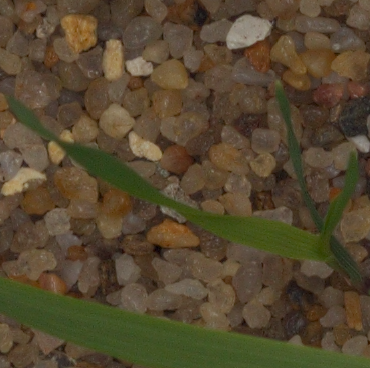
\includegraphics[width=30mm,height=30mm]{../figures/Black-grass_1af1eddd3.png} 
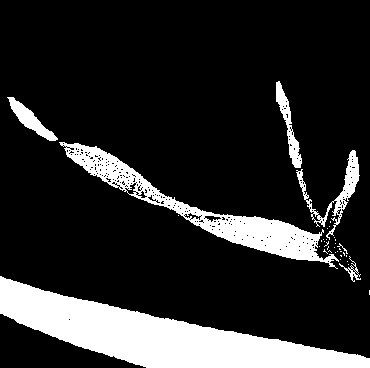
\includegraphics[width=30mm,height=30mm]{../figures/Black-grass_1af1eddd3_mask.png} 	
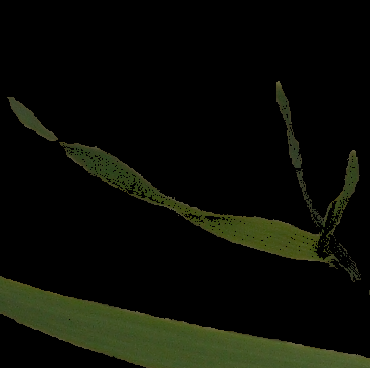
\includegraphics[width=30mm,height=30mm]{../figures/Black-grass_1af1eddd3_res.png} 
\caption{Black-grass的一个图像,其大小为$370\times 368$,从左到有依次为原图,掩膜图像,通过掩膜对原图过滤的图像}
\label{fig:bg1} 
\end{figure}

\begin{figure}[htbp]
\centering
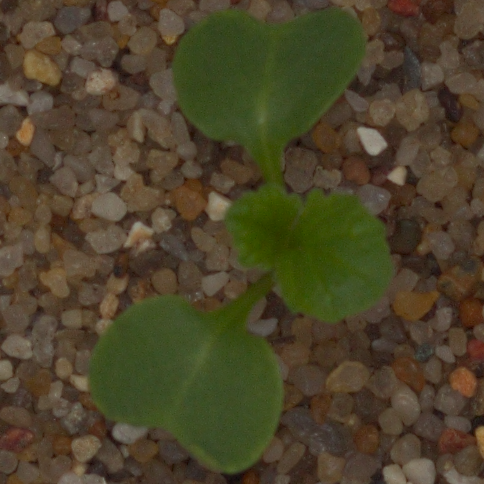
\includegraphics[width=30mm,height=30mm]{../figures/Charlock_0a7e1ca41.png} 
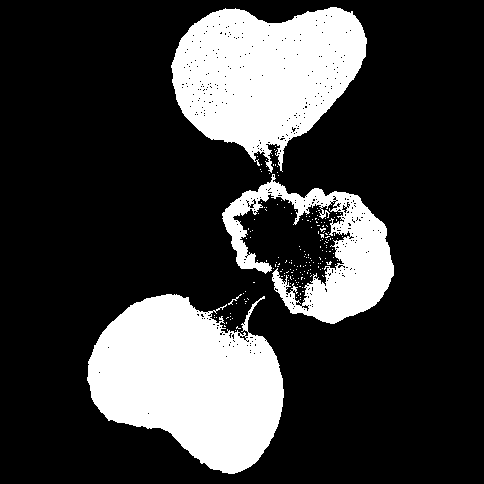
\includegraphics[width=30mm,height=30mm]{../figures/Charlock_0a7e1ca41_mask.png} 	
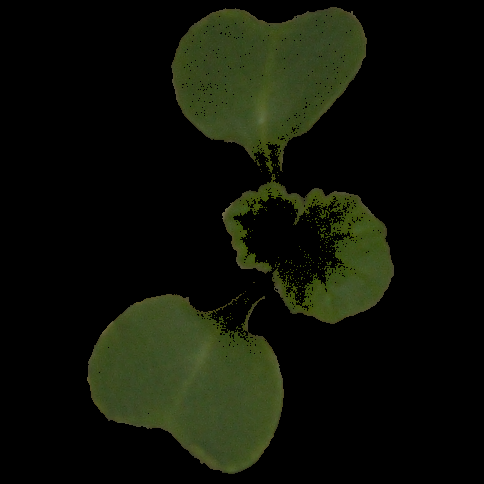
\includegraphics[width=30mm,height=30mm]{../figures/Charlock_0a7e1ca41_res.png} 	
\caption{Charlock的一个图像,其大小为$484\times 484$,从左到有依次为原图,掩膜图像,通过掩膜对原图过滤的图像}
\label{fig:ch1} 
\end{figure}

\begin{figure}[htbp]
\centering
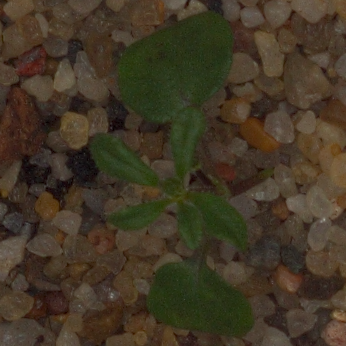
\includegraphics[width=30mm,height=30mm]{../figures/Cleavers_0a1e622bc.png} 
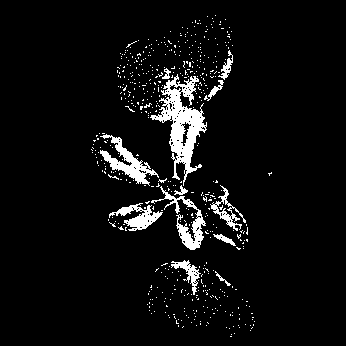
\includegraphics[width=30mm,height=30mm]{../figures/Cleavers_0a1e622bc_mask.png} 	
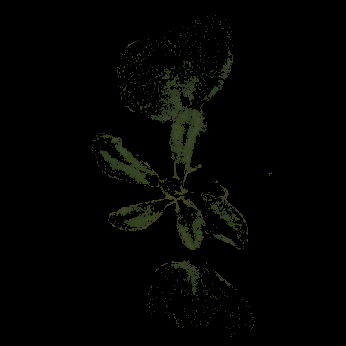
\includegraphics[width=30mm,height=30mm]{../figures/Cleavers_0a1e622bc_res.png} 
\caption{Cleavers的一个图像,其大小为$346\times 346$,从左到有依次为原图,掩膜图像,通过掩膜对原图过滤的图像}
\label{fig:cl} 
\end{figure}



\subsection{形态学去噪}
对于用掩模处理后的花苗二值图像,考虑到在花苗所在盆栽可能会有一些小草,通过掩模处理后会有噪声。因而考虑用形态学方法去噪。

对于一个二值图像,比较常用的去噪方法是形态学去噪,而这通常涉及两种形态学转换,分别为腐蚀和膨胀,其涉及的原理较简单。对于腐蚀,先定义一个窗口,窗口将沿着图像滑动,以遍历整个图像。滑动过程中,窗口内所有像素不全为1时,则令窗口中的所有像素等于0;若窗口内所有像素全为1,时,则不做操作。选用一个合适尺寸的窗口,对于腐蚀之后的图片,其白噪声点可以消除,但也会对物体的边缘进行腐蚀。膨胀则与腐蚀相反,区别在于滑动过程中,窗口内元素只要有1,则整个窗口元素都令为1,这样会增大物体的尺寸。通常对于有白噪声的图片,先腐蚀再膨胀可以消除白噪声,但一定程度会导致物体失真。但由于用掩模处理后的图像,其物体十分明显,用形态学方法去噪后失真的可能性不大。因而考虑用形态学方法去噪。
\subsection{边框裁剪与尺寸统一化}
我们从掩膜图像可以看出,目标图像(白色部分)只是占所有图像的很小一部分,而其余其余部分为黑色,而这其余的部分往往是无效的。现在考虑用一个矩形边框去提取出图像的有效区域,而将无效区域剔除。方法是访问图像中有效区域的宽度最小值和最大值,以及高度最小值和最大值,从而确定矩形边框区域。其效果图~\ref{fig:bycj}所示
\begin{figure}[htbp]
\centering
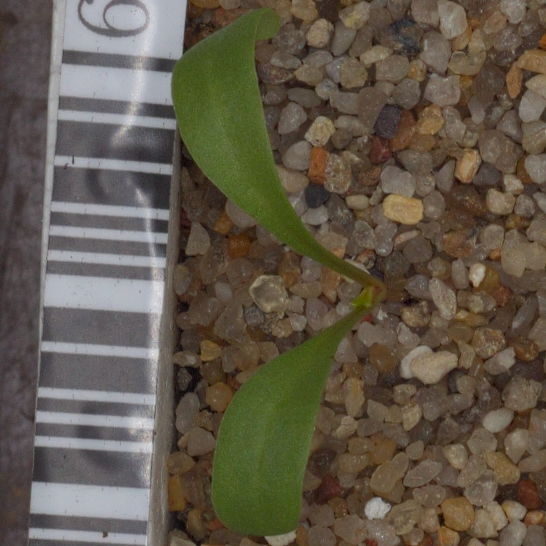
\includegraphics[width=30mm,height=30mm]{../figures/Sugar_beet_1bdfd2206.png} 
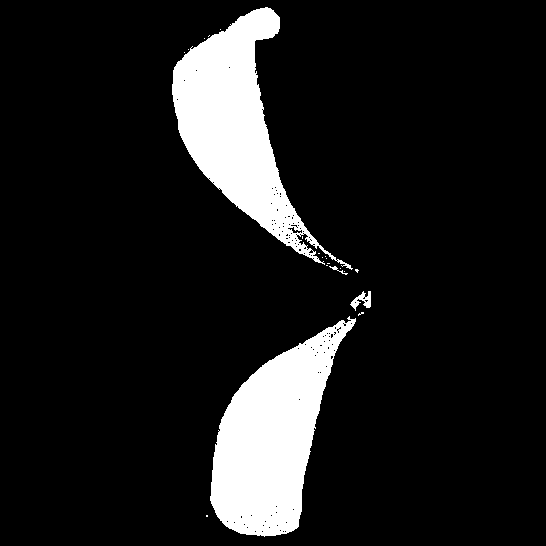
\includegraphics[width=30mm,height=30mm]{../figures/Sugar_beet_1bdfd2206_mask.png} 	
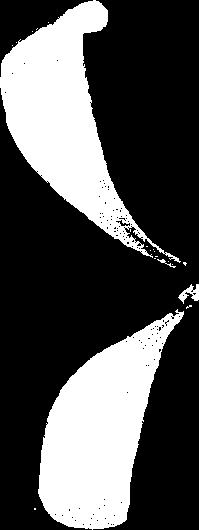
\includegraphics[width=10mm,height=30mm]{../figures/Sugar_beet_1bdfd2206_mask_tg.png}
\caption{Sugar beet的一个图像,其大小为$546\times 546$,从左到有依次为原图,掩膜图像,对掩膜图像矩形裁剪之后的图像,其大小为$199\times 530$}
\label{fig:bycj} 
\end{figure}

实现这个效果的代码如下
\begin{lstlisting}[language=python]
import cv2
# 获得矩形边框的最小宽高以及宽度和高度
x,y,w,h = cv2.boundingRect(mask_temp)
# 在原掩膜图像中选取矩形边框
mask_tg = mask[y:(y+h),x:(x+w)]
\end{lstlisting}
由于卷积神经网络需要同样大小尺寸的输入,所以考虑将图像统一尺寸归一化为统一的大小。内插的方法是INTER-CUBIC,其结果如图~\ref{fig:gyhW}

\begin{figure}[htbp]
\centering 
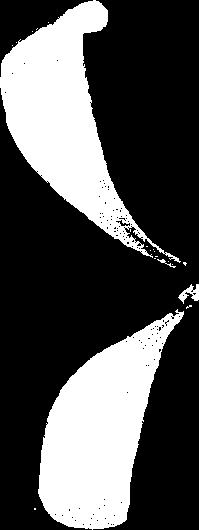
\includegraphics[width=10mm,height=30mm]{../figures/Sugar_beet_1bdfd2206_mask_tg.png} 	
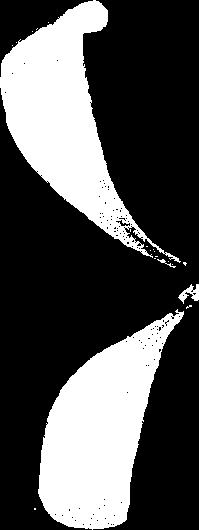
\includegraphics[width=30mm,height=30mm]{../figures/Sugar_beet_1bdfd2206_mask_tg.png} 	\\
\caption{Sugar beet的一个图像,左边为矩形裁剪之后的图像,大小为$199\times 530$,右边为尺寸统一化后的图像,大小为$96\times 96$}
\label{fig:gyh}
\end{figure}

实现这个效果的代码如下
\begin{lstlisting}[language=python]
import cv2
# 尺寸变换
mask_tg_rs = cv2.resize(mask_tg,[96,96],interpolation=cv2.INTER_CUBIC)
\end{lstlisting}
最后,对所有的图片都做上述操作。每张图片的掩膜的尺寸归一后的图像作为输入,需要注意的是,图片格式为uint8,需要转化为float才不会出问题,用以下代码可以解决该问题。
\begin{lstlisting}[language=python]
from skimage import img_as_float
imginput = img_as_float(mask_tg_rs) 
\end{lstlisting}

制作训练模型所需的数据集时,对原有的图片输入,通过以上变换之后所得到的imginput作为数据集的输入,而对原有的图片的名字进行one-hot编码处理作为数据集的输出。采用自助法分割训练集和验证集。训练集和验证集的样本数量比为$7:3$。在制备数据集输入时,制备三种规格分别为$64\times64$,$96\times96$,$128\times128$的数据集输入,而数据集输出不变,以探究不同大小的图片输入对神经网络性能的影响。为了方便表示,将上面三种规格的数据分别命名为I64,I96,I128,如表~\ref{table:t0}所示



\begin{table}[htbp]
\centering
\caption{训练集与验证集的构成}
\label{table:t0} 
\begin{tabular}{cccc}
\toprule[2pt] 
数据集名称 & 数据集用途 & 输入的数据特征 & 输出的数据特征 \\ 
\midrule[2pt]
\multirow{2}{*}{I64} & 训练集 & $3325,64,64,1$ & $3325,10$ \\ 
 & 验证集 & $1425,64,64,1$ & $1425,10$ \\ 
\midrule[1pt]
\multirow{2}{*}{I96} & 训练集 & $3325,96,96,1$ & $3325,10$ \\ 
 & 验证集 & $1425,96,96,1$ & $1425,10$ \\ 
\midrule[1pt]
\multirow{2}{*}{I128} & 训练集 & $3325,128,128,1$ & $3325,10$ \\ 
 & 验证集 & $1425,128,128,1$ & $1425,10$ \\ 
\bottomrule[2pt]
\end{tabular} 
\end{table}



